%%%%%%%%%%%%%%%%%%%%%% Generalities %%%%%%%%%%%%%%%%%%5
\documentclass[11pt,fleqn]{amsart}
%\usepackage[paper=a4paper]
 %{geometry}

\pagestyle{plain}
\pagenumbering{arabic}
%%%%%%%%%%%%%%%%%%%%%%%%%%%%%%%%
\usepackage[small]{titlesec}
\usepackage{hyperref}
\usepackage{amsthm,thmtools}
%\usepackage{showlabels}
\linespread{1.05}
%\setlength{\parskip}{1.2ex}

\usepackage[utf8]{inputenc}
\usepackage[english]{babel}
\usepackage{enumerate}
\usepackage[osf,noBBpl]{mathpazo}
\usepackage[alphabetic,initials]{amsrefs}
\usepackage{amsfonts,amssymb,amsmath}
\usepackage{mathtools}
\usepackage{graphicx}
\usepackage[poly,arrow,curve,matrix]{xy}
%\usepackage{wrapfig}
%\usepackage{xcolor}
\usepackage{helvet}
\usepackage{stmaryrd}
\usepackage{tikz}
\usepackage{mathdots}
%\usepackage[normalem]{ulem}

\renewcommand\thesection{\arabic{section}}
\titleformat{\section}
 {\normalfont\bfseries\large}
 {\thesection. \space}{0em}{}

\renewcommand\thesubsection{\arabic{subsection}}
\titleformat{\subsection}
 {\normalfont\bfseries}
 {\thesection.\thesubsection \space}{0em}{}

\renewcommand\proofname{Proof}

\makeatletter
\renewenvironment{proof}[1][\textit{\proofname}]{\par
 \pushQED{\qed}%
 \normalfont \topsep.75\paraskip\relax
 \trivlist
 \item[\hskip\labelsep
 \itshape
 #1\@addpunct{.}]\ignorespaces
}{%
 \popQED\endtrivlist\@endpefalse
}
\makeatother
%%%%%%%%%%%%%%%%%%%%%%%%%%% Theorems et al%%%%%%%%%%%%%%%%%%%%%%%%%%
\declaretheoremstyle[
%headformat=swapnumber, 
bodyfont=\itshape,]{mystyle}
\declaretheorem[name=Lemma, style=mystyle, numberwithin=section]{Lemma}
\declaretheorem[name=Proposition, style=mystyle, sibling=Lemma]{Proposition}
\declaretheorem[name=Theorem, style=mystyle, sibling=Lemma]{Theorem}
\declaretheorem[name=Corollary, style=mystyle, sibling=Lemma]{Corollary}
\declaretheorem[name=Definition, style=mystyle, sibling=Lemma]{Definition}
\declaretheorem[name=Example, style=mystyle, sibling=Lemma]{Example}
\declaretheorem[name=Remark, style=mystyle, sibling=Lemma]{Remark}

% unnumbered versions
\declaretheoremstyle[numbered=no, 
bodyfont=\itshape]{mystyle-empty}
\declaretheorem[name=Lemma, style=mystyle-empty]{Lemma*}
\declaretheorem[name=Proposition, style=mystyle-empty]{Proposition*}
\declaretheorem[name=Theorem, style=mystyle-empty]{Theorem*}
\declaretheorem[name=Corollary, style=mystyle-empty]{Corollary*}
\declaretheorem[name=Definition, style=mystyle-empty]{Definition*}
\declaretheorem[name=Example, style=mystyle-empty]{Example*}
\declaretheorem[name=Remark, style=mystyle-empty]{Remark*}

%%%%%%%%%%%%%%%%%%%%%%%%%%% Paragraphs %%%%%%%%%%%%%%%%%%%%%%%%%%%%%
\newskip\paraskip
\paraskip=0.75ex plus .2ex minus .2ex

\newcounter{para}[section]
\setcounter{para}{0}
\renewcommand\thepara{\thesection.\arabic{para}}
\def\paragraph{%
 \noindent
 \refstepcounter{para}%
 \textbf{\thepara.}\hspace{1ex}%
}

\newcommand\about[1]{%
 {\bfseries#1.}%
}

\newcommand\pref[1]{\textbf{\ref{#1}}}

\renewcommand\theHpara{\theHsection.\arabic{para}}
%%%%%%%%%%%%%%%%%%%%%%%%%%% The usual stuff%%%%%%%%%%%%%%%%%%%%%%%%%
\newcommand\NN{\mathbb N}
\newcommand\CC{\mathbb C}
\newcommand\QQ{\mathbb Q}
\newcommand\RR{\mathbb R}
\newcommand\ZZ{\mathbb Z}
\renewcommand\k{\Bbbk}

\newcommand\maps{\longmapsto}
\newcommand\ot{\otimes}
\renewcommand\to{\rightarrow}
\renewcommand\phi{\varphi}
\newcommand\id{\mathsf{Id}}
\newcommand\im{\mathsf{im}}
\newcommand\coker{\mathsf{coker}}
%%%%%%%%%%%%%%%%%%%%%%%%% Specific notation %%%%%%%%%%%%%%%%%%%%%%%%%
%\newcommand\II{\mathcal I}
%\newcommand\II'{\mathcal J}

\newcommand\g{\mathfrak g}
\newcommand\p{\mathfrak p}
\newcommand\m{\mathfrak m}
\newcommand\gl{\mathfrak{gl}}
\renewcommand\sl{\mathfrak{sl}}
\newcommand\vv{\overline{v}}
\newcommand\II{\mathbb I}
\newcommand\RI{\overline{\mathbb I}}
\newcommand\GT{\mathcal{GT}}

\newcommand\vectspan[1]{\left\langle #1 \right\rangle}
\newcommand\interval[1]{\llbracket #1 \rrbracket}
\newcommand\abs[1]{|#1|}

\DeclareMathOperator\Frac{Frac}
\DeclareMathOperator\Specm{Specm}
\DeclareMathOperator\End{End}
\DeclareMathOperator\Hom{Hom}

\DeclareMathOperator\sym{sym}
\DeclareMathOperator\asym{asym}
\DeclareMathOperator\sg{sg}
\DeclareMathOperator\ev{\mathsf{ev}}
\DeclareMathOperator\supp{supp}
\DeclareMathOperator\essupp{essupp}

\newcommand\DD{\mathbb D}
\newcommand\D{\mathfrak D}
\newcommand\bigmodule{big GT module~}

\renewcommand\labelitemi{--}

%%%%%%%%%%%%%%%%%%%%%%%%%%%%%%%%%%%%%% TITLES %%%%%%%%%%%%%%%%%%%%%%%%%%%%%%
\title{Children of big Gelfand-Tsetlin modules}
%\author{[structure.tex]}
\date{}


\begin{document}
\maketitle
%\vspace{-2cm}
\section{Combinatorial preliminaries}

\paragraph
\about{Notation}
\label{notation}
Given $a,b,k \in \NN$ we set $\interval{a,b} = \{i \in \NN \mid a \leq i \leq 
b\}$ and $\interval{b} = \interval{1,b}$. Also we denote by $S_k$ the 
symmetric group in $k$-elements, and given $\pi = (\pi_1, \ldots, \pi_r)$
with $\sum_i \pi_i = k$ we denote by $S_\pi$ the product of symmetric groups
$S_{\pi_1} \times S_{\pi_2} \times \cdots \times S_{\pi_r}$, seen in the 
natural way as subgroup of $S_k$.

Fix $n \in \NN$ and let $\mu = (1, 2, \ldots, n)$. Given $\sigma \in S_\mu$ we 
write $\sigma_{(k)}$ for its projection to $S_k$. We make a slight abuse of 
notation, and identify $S_k$ with the subgroup of $S_\mu$ consisting of 
elements such that $\sigma_{(i)}$ is the identity for all $i \neq k$. Thus we 
can write $\sigma = \sigma_{(1)} \sigma_{(2)} \cdots \sigma_{(n)}$.

The group $S_\mu$ is a Coxeter group with generating set $\{(i,i+1)_{(k)}
\mid k \in \interval{n}, i \in \interval{k-1}\}$. The usual notions of length,
Bruhat order, parabolic subgroups, etc. will be considered with respect to 
this generating set. In particular the length of $\sigma \in S_\mu$ is equal 
to $\ell(\sigma) = \ell_1(\sigma_{(1)}) + \cdots + \ell_n(\sigma_{(n)})$, 
where $\ell_k$ is the usual notion of length in $S_k$. Also $\sigma < \tau$ in 
the Bruhat order if and only if $\sigma_{(k)} < \tau_{(k)}$ for all $k$.

Set $\Sigma = \{(k,i) \mid 1 \leq i \leq k \leq n\}$. The group $S_\mu$ acts 
on $\Sigma$ with the action given by $\sigma \cdot (k,i) = (k, 
\sigma_{(k)}(i))$. The subset $\Sigma' = \{(k,i) \mid 1 \leq i \leq k \leq n-1
\}$ is clearly invariant by this action. 

Given $a \leq b \leq k$ we set $\interval{a,b}_k = \{(k,i) \mid i \in 
\interval{a,b}\} \subset \Sigma$. Such a set will be called an \emph{interval}
of $\Sigma$, and given an interval $I = \interval{a,b}_k$ we write $a(I) = a,
b(I) = b, k(I) = k$. A partition of $\Sigma$ is a family of nonempty subsets 
of $\Sigma$, which we cal \emph{blocks}, whose disjoint union is $\Sigma$.
An \emph{interval partition} is a partition $\II$ whose blocks are intervals. 
We write $\II[k]$ for the set of all intervals $I \in \II$ with $k(I) = k$. 
We denote by $S(\II)$ the subgroup of $S_\mu$ stabilizing the blocks of $\II$,
which is a parabolic subgroup of $S_\mu$.

\paragraph
Let $\CC^\mu = \CC \times \CC^2 \times \cdots \times \CC^n$, so $v \in \CC^\mu$
is an $n$-tuple $(v_1, v_2, \ldots, v_n)$ with $v_k = (v_{k,1}, v_{k,2},
\ldots, v_{k,k}) \in \CC^k$. For each $(k,i) \in \Sigma$ we denote by 
$\delta^{k,i} \in \CC^\mu$ the unique element in $\CC^\mu$ such that 
$\delta^{k,i}_{l,j} = \delta_{k,l} \delta_{i,j}$, and refer to the set 
$\{\delta^{k,i}\mid (k,i) \in \Sigma\}$ as the canonical basis of $\CC^\mu$. 
The group $S_\mu$ acts on $\CC^\mu$ by linear operators whose action on the 
canonical basis is given by $\sigma \cdot \delta^{k,i} = \delta^{\sigma \cdot 
(k,i)} = \delta^{k, \sigma_{(k)} (i)}$. We denote by $\ZZ^\mu_0$ the abelian 
group generated by $\{\delta^{k,i} \mid (k,i) \in \Sigma'\}$, which is 
clearly stable by the action of $S_\mu$.

Given $v \in \CC^\mu$ we construct a graph $\Omega(v)$ as follows. The set of 
vertices of $\Omega(v)$ is $\{[k,i] \mid (k,i) \in \Sigma\}$, and we have an 
edge between $[k,i]$ and $[l,j]$ if and only if $v_{k,i} - v_{l,j} \in \ZZ$ 
and $|k-l| \leq 1$. We will write $[k,i] - [l,j]$ as an abbreviation of 
``an edge between $[k,i]$ and $[l,j]$'' (we use square brackets to denote 
vertices so there is less chance of confusing this symbol with a 
substraction). We say two vertices are connected if they lie in the same 
connected component of $\Omega(v)$. 

Given an interval $I = \interval{a,b}_k$ we will write $v(I)$ for $(v_{k,a}, 
v_{k,a+1}, \cdots, v_{k,b})$. Given an interval partition $\II$ of $\Sigma$ we 
refer to the tuples $v(I)$ with $I \in \II$ as the blocks of $v$. We 
associate with $v$ a partition of $\Sigma$ denoted by $\II(v)$, where the 
block of $(n,i)$ is $\{(n,i)\}$, and for $k < n$ the block of $(k,i)$ is the 
set of all $(k,j)$ such that $[k,i] - [k,j]$ is an edge in $\Omega(v)$.

\begin{Definition}
We say that $v \in \CC^\mu$ is in \emph{normal form} if whenever $[k,a] - 
[k,b]$ is an edge of $\Omega(v)$ and $a \leq i < j \leq b$, then
$v_{k,i} - v_{k,j} \in \ZZ_{\geq 0}$. 
\end{Definition}
Notice that if $v$ is in normal form then $\II(v)$ is an interval partition.
Clearly for each $v \in \CC^\mu$ there exists at least one element in its 
$S_\mu$-orbit which is in normal form. 

Suppose $v$ is in normal form and let $\II(v)[k] = \{I_1, I_2, \ldots, I_r\}$, 
with $a(I_i) = b(I_{i-1}) + 1$. We set $\pi(v,k) = (\abs{I_1},\abs{I_2}, 
\ldots, \abs{I_r})$, so $S_{\pi(v,k)}$ is a parabolic subgroup of $S_k$; 
observe that by definition $S_{\pi(v,n)}$ is the trivial subgroup of $S_n$. 
We denote by $\pi(v)$ the concatenation of $\pi(v,1), \ldots, \pi(v,n)$, and 
set $S_{\pi(v)} = S_{\pi(v,1)} \times S_{\pi(v,2)} \cdots 
\times S_{\pi(v,n)} \subset S_\mu$, which a parabolic subgroup of $S_\mu$.
\begin{Definition}
We say that $\vv \in \CC^\mu$ is a \emph{seed} if it is in normal form and 
whenever $[k,i]$ and $[l,j]$ are connected in $\Omega(v)$ and $k,l < n$ then
$\vv_{k,i} = \vv_{l,j}$.
\end{Definition}
As mentioned above, $S_\mu$ acts on $\CC^\mu$ and $\ZZ_0^\mu$ is stable by
this action. Also $\ZZ_0^\mu$ acts on $\CC^\mu$ by translation, i.e. for each
$z \in \ZZ_0^\mu$ and each $v \in \CC^\mu$ we have $z \cdot v = v + z$. Thus 
the crossed product $\ZZ_0^\mu \# S_\mu$ acts on $\CC^\mu$. Clearly for every
$v \in \CC^\mu$ there exists a seed in its $\ZZ_0^\mu \# S_\mu$-orbit. Two 
elements $v,w \in \CC^\mu$ lie in the same orbit if and only if there exists
$\sigma \in S_\mu$ such that $\sigma(\Omega(v)) = \Omega(w)$, where $\sigma$
acts on the vertices of the graph in the obvious way.
\begin{Example}
We will write elements of $\CC^\mu$ as triangular arrays with $k$ entries in
its $k$-th row. In this and all other examples we assume that the set $\{1, a,
b, c, \ldots\} \subset \CC$ is linearly independent over $\ZZ$.

\begin{tabular}{cc}
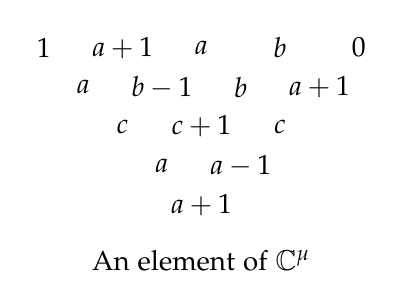
\begin{tikzpicture}
\node (51) at (-2,2.5) {$1$};
\node (52) at (-1,2.5) {$a+1$};
\node (53) at (0,2.5) {$a$};
\node (54) at (1,2.5) {$b$};
\node (55) at (2,2.5) {$0$};

\node (41) at (-1.5,2) {$a$};
\node (42) at (-0.5,2) {$b-1$};
\node (43) at (0.5,2) {$b$};
\node (44) at (1.5,2) {$a+1$};

\node (31) at (-1,1.5) {$c$};
\node (32) at (0,1.5) {$c+1$};
\node (33) at (1,1.5) {$c$};

\node (21) at (-.5,1) {$a$};
\node (22) at (.5,1) {$a-1$};

\node (11) at (0,0.5) {$a+1$};

\node (text) at (0,-0.2) {An element of $\CC^\mu$};
\end{tikzpicture}

&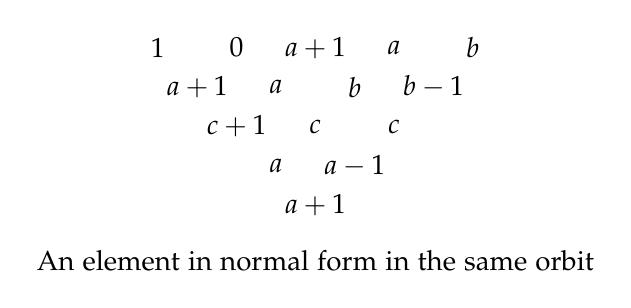
\begin{tikzpicture}
\node (51) at (-2,2.5) {$1$};
\node (52) at (-1,2.5) {$0$};
\node (53) at (0,2.5) {$a+1$};
\node (54) at (1,2.5) {$a$};
\node (55) at (2,2.5) {$b$};

\node (41) at (-1.5,2) {$a+1$};
\node (42) at (-0.5,2) {$a$};
\node (43) at (0.5,2) {$b$};
\node (44) at (1.5,2) {$b-1$};

\node (31) at (-1,1.5) {$c+1$};
\node (32) at (0,1.5) {$c$};
\node (33) at (1,1.5) {$c$};

\node (21) at (-.5,1) {$a$};
\node (22) at (.5,1) {$a-1$};

\node (11) at (0,0.5) {$a+1$};

\node (text) at (0,-0.2) {An element in normal form in the same orbit};
\end{tikzpicture} \\

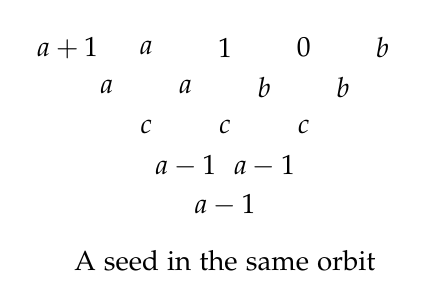
\begin{tikzpicture}
\node (51) at (-2,2.5) {$a+1$};
\node (52) at (-1,2.5) {$a$};
\node (53) at (0,2.5) {$1$};
\node (54) at (1,2.5) {$0$};
\node (55) at (2,2.5) {$b$};

\node (41) at (-1.5,2) {$a$};
\node (42) at (-0.5,2) {$a$};
\node (43) at (0.5,2) {$b$};
\node (44) at (1.5,2) {$b$};

\node (31) at (-1,1.5) {$c$};
\node (32) at (0,1.5) {$c$};
\node (33) at (1,1.5) {$c$};

\node (21) at (-.5,1) {$a-1$};
\node (22) at (.5,1) {$a-1$};

\node (11) at (0,0.5) {$a-1$};

\node (text) at (0,-0.2) {A seed in the same orbit};
\end{tikzpicture}
&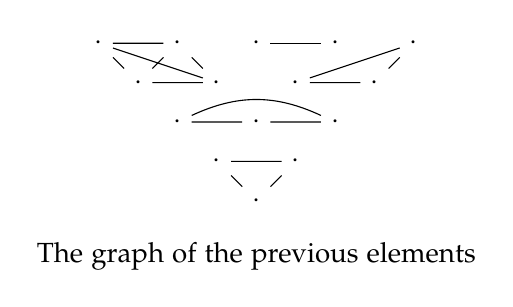
\begin{tikzpicture}
\node (51) at (-2,2.5) {$\cdot$};
\node (52) at (-1,2.5) {$\cdot$};
\node (53) at (0,2.5) {$\cdot$};
\node (54) at (1,2.5) {$\cdot$};
\node (55) at (2,2.5) {$\cdot$};

\node (41) at (-1.5,2) {$\cdot$};
\node (42) at (-0.5,2) {$\cdot$};
\node (43) at (0.5,2) {$\cdot$};
\node (44) at (1.5,2) {$\cdot$};

\node (31) at (-1,1.5) {$\cdot$};
\node (32) at (0,1.5) {$\cdot$};
\node (33) at (1,1.5) {$\cdot$};

\node (21) at (-.5,1) {$\cdot$};
\node (22) at (.5,1) {$\cdot$};

\node (11) at (0,0.5) {$\cdot$};

\node (text) at (0,-0.2) {The graph of the previous elements};

\draw (51) -- (52) -- (42) -- (41) -- (51) -- (42) (52) -- (41);
\draw (53) -- (54);
\draw (55) -- (43) -- (44) -- (55);
\draw (31) -- (32) -- (33) to[out=155,in=25] (31);
\draw (11) -- (21) -- (22) -- (11);
\end{tikzpicture}
\end{tabular}
\end{Example}

\paragraph
\label{descending-z}
\about{Descending $\II$-sequences}
Recall that we denote by $\ZZ^\mu_0$ the set of all $z \in \CC^\mu$ with
$z_{k,i} \in \ZZ$ for all $(k,i) \in \Sigma'$ and $z_{n,i} = 0$ for all $n$.
\begin{Definition}
Let $\vv \in \CC^\mu$ be a seed. We denote by $\DD(\vv)$ the set of all
$z \in \ZZ_0^\mu$ such that such that $z(I)$ is a decreasing sequence for all 
$I \in \II(\vv)$.
\end{Definition}
If $\vv$ is a seed then $\DD(\vv)$ is exactly the set of those $z \in 
\ZZ_0^\mu$ such that $\vv + z$ is in normal form. For the rest of this section 
we fix a seed $\vv$ and set $\II = \II(\vv)$ and $\pi = \pi(\vv)$.
Let $z \in \DD(\vv)$. The stabilizer of $z$ in $S_\pi$ is again a parabolic 
subgroup of $S_\pi$, which we denote as usual by $(S_\pi)_z$. Thus each 
coclass in $S_\pi/(S_\pi)_z$ has a unique minimal length representative. We 
denote by $S_\pi^z$ the set of these minimal length representatives, and refer 
to them as \emph{$z$-shuffles}. Given $\sigma \in S_\pi$ we denote by 
$\sigma^z$ the unique $z$-shuffle in $\sigma S_\pi$.

We denote by $\II(\vv,z)$ the interval partition of $\Sigma$ where $(k,i)$ and 
$(k,j)$ lie in the same block if and only if they lie in the same block of 
$\II(\vv)$ and $z_{k,i} = z_{k,j}$. Equivalently, $\II(\vv,z)$ is the unique
interval partition of $\Sigma$ such that $(S_\pi)_z = S(\II(\vv, z))$. 
Let us say that $\sigma \in S_\pi$ is increasing over an interval 
$\interval{a,b}_k \subset \Sigma$ if $\sigma_{(k)}(i) < \sigma_{(k)}(j)$ 
whenever $a \leq i < j \leq b$. A permutation is a $z$-shuffle if and only if 
it is increasing over every interval in $\II(\vv, z)$, so $\sigma^z$ is the 
unique permutation in $S_\pi$ increasing over all intervals in $\II(\vv, z)$ 
and such that $\sigma^z(z) = \sigma(z)$.

Given an interval $I = \interval{a,b}_k$ we denote by $\omega(I)$ the 
permutation $i \mapsto  b+a-i$. This is the longest element in the symmetric
group of the interval $I$, seen as a subgroup of $S_\mu$. It follows 
that if $\II$ is an interval partition then the longest element in $S(\II)$ is 
$\prod_{I\in\II} \omega(I)$. We also write $\alpha(I)$ for the permutation 
$(b \ b-1)_{(k)} (b-1 \ b-2)_{(k)} \cdots (a-1 \ a)_{(k)}$ and $\beta(I)$ for 
its inverse, namely $(a \ a+1)_{(k)} (a+1 \ a+2)_{(k)} \cdots(b-1 \ b)_{(k)}$. 
\begin{Lemma}
\label{L:omega-delta}
Let $z\in \DD(\vv)$ and let $\omega_0$ be the longest element in $S_\pi$.
\begin{enumerate}[(a)]
\item 
\label{i:omega-z}
We have $\omega_0^z = \omega_0 \prod_{I \in \II(\vv, z)} \omega(I)$.

\item 
\label{i:D-delta}
Given $(k,i) \in \Sigma$, we have $z + \delta^{k,i} \in \DD(\vv)$ if and only 
	if $i = a(I)$ for some $I \in \II(\vv,z)[k]$. Analogously, $z-\delta^{k,i} 
	\in \DD(\vv)$ if and only if $i = b(I)$ for some $I \in \II(\vv,z)[k]$.

\item 
\label{i:omega-delta}
Let $I = \interval{a,b}_k \in \II(\vv,z)$ and set $u=z+\delta^{k,a}, 
	v = z- \delta^{k,b}$. There exist $\sigma, \tau \in S_\pi^z$ such that 
	$\omega_0^u = \sigma \alpha(I)$ and $\omega_0^v = \tau \beta(I)$. 
\end{enumerate}
\end{Lemma}
\begin{proof}
Put $\II' = \II(\vv,z)$.
By definition $\omega_0$ reverses the order of each interval $I$ in $\II'$. 
Since $\omega(I)$ is decreasing over $I$, it follows that $\omega_0 \prod_{I 
\in \II'} \omega(I)$ is increasing over every interval $I \in \II'$, so it is 
a $z$-shuffle lying in the coclass $\omega_0 (S_\pi)_z$. This proves item 
\ref{i:omega-z}. Item \ref{i:D-delta} follows immediately from the 
definitions. 

To prove item \ref{i:omega-delta} we will show the equivalent statement that  
$\sigma = \omega_0^u \beta(I)$ and $\tau = \omega_0^v \alpha(I)$ are 
$z$-shuffles. We check this in the first case, the
second can be checked analogously. Let $J$ be the interval in $\II(\vv,u)$
corresponding to $(k,a)$, so $J = \interval{c,a}_k$ for some $c \leq a$. Set
$J' = J \setminus \{(k,a)\}$ and $I' = I \setminus \{(k,a)\}$, then by item
\ref{i:omega-z}
\begin{align*}
\omega_0^u \beta(I)
	&= \omega_0 \left( \prod_{K \in \II(\vv, u), K \neq I',J} \omega(K) \right)
		\omega(J)\omega(I')\beta(I) \\
	&= \omega_0 \left( \prod_{K \in \II(\vv, z), K \neq I,J'} \omega(K) \right)
		\omega(J)\omega(I')\beta(I).
\end{align*}
It is enough to check that the composition of the product in parenthesis with 
$\omega(J)\omega(I')\beta(I)$ is decreasing over the intervals of 
$\II(\vv,z)$. This is immediate for $K \neq I, J'$, so all we have to 
do is check that $\omega(J)\omega(I')\beta(I)$ is decreasing over $I, J'$, and 
this is easy to do. A similar reasoning shows that $\tau$ is a $z$-shuffle.
\end{proof}

\section{Big Gelfand-Tsetlin modules and their submodules}
Throughout this section we fix a seed $\vv$ and set $\II = \II(\vv), \pi = 
\pi(\vv)$.

\paragraph
\about{Gelfand-Tsetlin modules}
For each $k \in \interval{n}$ we denote by $U_k$ the enveloping algebra of 
$\gl(k,\CC)$, and set $U = U_n$. Inclusion of matrices in the top left corner 
induces a chain
\begin{align*}
\gl(1,\CC) \subset \gl(2, \CC) \subset \cdots \subset \gl(n,\CC),
\end{align*}
which in turn induces a chain $U_1 \subset U_2 \subset \cdots \subset U_n$. 
Denote by $Z_k$ the center of $U_k$ and by $\Gamma$ the subalgebra of $U$ 
generated by $\bigcup_{k=1}^n Z_k$. This algebra is the \emph{Gelfand-Tsetlin} 
subalgebra of $U$, and it is generated by the elements
\begin{align*}
c_{k,i}
  &= \sum_{(r_1, \ldots, r_i) \in \interval{k}^i} 
    E_{r_1, r_2} E_{r_2, r_3} \cdots E_{r_i, r_1},
  & (k,i) \in \Sigma.
\end{align*}
By work of Zhelobenko there exists an isomorphism $\Gamma \to \CC[x_{k,i} 
\mid (k,i) \in \Sigma]^{S_\mu}$, given by $c_{k,i} \mapsto 
\gamma_{k,i}$ where
\begin{align*}
\gamma_{k,i}
  &= \sum_{j=1}^k (x_{k,j} + k - 1)^i 
    \prod_{m \neq j} \left( 
      1 - \frac{1}{x_{k,j} - x_{k,m}}
    \right),
\end{align*}
see \cite{FGR16}*{Subsection 3.1} for details. We will denote the image of 
$c \in \Gamma$ through this isomorphism by $\gamma_c$.
It follows that $\Specm \Gamma \cong \CC^\mu / S_\mu$, and so every 
$v \in \CC^\mu$ induces a character $\chi_v: \Gamma \to \CC$ by setting
$c \in \Gamma \mapsto \gamma_c(v)$. 
\begin{Definition*}
A $U$-module $M$ is called a \emph{Gelfand-Tsetlin module} if it is finitely
generated and
\[
  M = \bigoplus_{\m \in \Specm \Gamma} M[\mathfrak m],
\] 
where $M[\mathfrak m] = \{x \in M \mid \mathfrak m^k x = 0 \mbox{ for some } k 
\geq 0\}$. The \emph{support} of $M$ is the set of all $\m$ such that $M[\m]
\neq 0$. If $\m$ lies in the support of $M$ then its \emph{multiplicity} is
$\dim M[\m]$.
\end{Definition*}
Let $M$ be a Gelfand-Tsetlin module and let $v \in \CC^\mu$. We put
$M[v] = M[\ker \chi_v]$, and denote by $p_v: M \to M[v]$ the natural projection
map. We will identify the support of $M$ with the set of all $v \in \CC^\mu$ 
such that $M[v] \neq 0$. We will often abbreviate Gelfand-Tsetlin by GT, or 
ommit it completely when it is clear from the context.

It is easy to check that $M$ is a Gelfand-Tsetlin module if and only if for 
each $m \in M$ the complex vector space $\Gamma m$ has finite dimension. The
following lemma is an immediate consequence.
\begin{Lemma}
\label{L:sub-gt}
Let $M$ be a Gelfand-Tsetlin module and let $N \subset M$ be a $U$-submodule.
Then $N$ is also a Gelfand-Tsetlin module. In particular for each $x \in N$
we have $p_v(n) \in N$ for all $v \in \CC^\mu$.
\end{Lemma}

Denote by $\GT$ the category of all Gelfand-Tsetlin modules, and for each 
equivalence class $\zeta \in \CC^\mu / (\ZZ_0^\mu \# S_\mu)$ denote by 
$\GT_\zeta$ the full subcategory of all Gelfand-Tsetlin modules whose support 
is contained in $\zeta$. According to \cite{FO14}*{Corollary 3.4} we get a 
decomposition
\begin{align*}
\GT &= \bigoplus_{\zeta \in  \CC^\mu / (\ZZ_0^\mu \# S_\mu)} \GT_\zeta
\end{align*}
so the determination of simple objects of $\GT$ is reduced to the determination
of the simple objects of each $\GT_\zeta$. 

\paragraph
\about{Big Gelfand-Tsetlin modules}
\label{big-gt-modules}
There exists a Gelfand-Tsetlin module, denoted by $V(T(\vv))$, whose support 
equals $\vv + \DD(\vv)$; this module was first introduced in \cite{RZ18} 
(see also \cite{EMV18}, which came out at the same time). Its component of 
weight $\vv + z$ has a basis $\{D_\sigma(\vv+z) \mid \sigma \in S_\pi^z\}$, 
whose elements are called \emph{derived tableaux}. A tableau of the form 
$D_e(\vv + z)$ is called the \emph{classical tableaux} associated to $\vv + z$.
Given $z \in \DD(\vv)$ and $\sigma \in S_\pi^z$ we denote by $D_{<\sigma}(\vv 
+ z)$ an arbitrary linear combination of tableaux $D_\tau(\vv + z)$ with 
$\tau \in S_\pi^z$ strictly smaller than $\sigma$ in the induced Bruhat order
(for details regarding the Bruhat order on shuffles see 
\cite{BB05}*{Section 2.5}). 

The action of $U = U(\gl(n,\CC))$ on $V(T(\vv))$ was described in 
\cite{FGRZ18}. We review the main results. Given $I = \interval{a,b}_k$ with 
$k <n$ we set
\begin{align*}
e_I
	&= \frac{\displaystyle \prod_{j = 1}^{k+1} x_{k,a} - x_{k+1,j}}
		{\displaystyle \prod_{(k,j) \notin I} x_{k,a} - x_{k,j}};
&f_I
	&= \frac{\displaystyle \prod_{j = 1}^{k-1} x_{k,b} - x_{k-1,j}}
		{\displaystyle \prod_{(k,j) \notin I} x_{k,b} - x_{k,j}}.
\end{align*}
Notice that if $I \in \II(\vv,z)$ then $e_I(\vv + z)$ and $f_I(\vv + z)$ are
well defined. We also set 
\begin{align*}
h_k = x_{k,1} + \cdots + x_{k,k} - (x_{k-1, 1} + \cdots + x_{k-1,k-1}) + k - 1.
\end{align*}

The following theorem is a direct consequence of \cite{FGRZ18}*{Lemma 8.4}.
\begin{Theorem}
\label{T:gt-big-module}
The action of the canonical generators of $\gl(n,\CC)$ on $V(T(\vv))$ is given 
by
\begin{align*}
E_{k,k+1} D_\sigma(\vv + z) &= 
%	&= - \sum_{I \in \II(\vv,z)[k]} 
%		\sum_{\tau < \sigma \alpha(I)} 
%			\D_{\tau,\sigma\alpha(I)}^{\vv + z}(e_{I})
%			D_{\tau}(\vv + z + \delta^{k,a(I)}) \\
	 - \sum_{I \in \II(\vv,z)[k]} \bigg(
		e_I(\vv + z) D_{\sigma\alpha(I)}(\vv+z + \delta^{k,a(I)})\\
			&\qquad\qquad + D_{<\sigma\alpha(I)}(\vv+z + \delta^{k,a(I)})
			\bigg) \\
E_{k+1,k} D_\sigma(\vv + z) &=
%	&= \sum_{I \in \II(\vv,z)[k]} 
%		\sum_{\tau < \sigma \beta(I)} 
%			\D_{\tau,\sigma\beta(I)}^{\vv + z}(f_{I})
%			D_{\tau}(\vv + z - \delta^{k,b(I)}) \\
	\sum_{I \in \II(\vv,z)[k]} \bigg(
		f_I(\vv + z) D_{\sigma\beta(I)}(\vv + z - \delta^{k,b(I)}) \\
			&\qquad\qquad
			+  D_{<\sigma\beta(I)}(\vv + z - \delta^{k,b(I)})
			\bigg)\\
E_{k,k} D_{\sigma}(\vv + z) 
	&= h_k(\vv + z) D_{\sigma}(\vv+z). 
\end{align*}
\end{Theorem}

The following proposition describes the weight components of $V(T(\vv))$. 
Proofs for these results can be found in \cite{FGRZ18}*{Proposition 6.4 and
Lemma 6.5}.
\begin{Proposition}
\label{P:gt-weight-spaces}
Let $z \in \DD(\vv)$ and set $T = \sum_\sigma a_\sigma D_\sigma(\vv + z)$.
\begin{enumerate}[(a)]
\item 
\label{i:action}
If $c \in \Gamma$ then
\begin{align*}
c D_\sigma(\vv + z)
	&= \gamma_c(\vv+z)D_\sigma(\vv+z) +
		\sum_{\tau < \sigma} \D_{\tau,\sigma}^{\vv + z}(\gamma_c) 
			D_\tau(\vv+z)\\
	&= \gamma_c(\vv+z)D_\sigma(\vv+z) + D_{<\sigma}(\vv+z).
\end{align*}

\item 
\label{i:generator}
The element $T$ generates the component of Gelfand-Tsetlin weight $\vv+z$
if and only if $a_{\omega_0^z} \neq 0$.

\item 
\label{i:eigenvalue}
If $(c - \gamma(c))^r T = 0$ for all $c \in \Gamma$ then $a_\sigma = 0$
whenever $\ell(\sigma) \geq r$. In particular the space of eigenvectors with
eigenvalue $\chi_{\vv + z}$ is generated by $D_e(\vv + z)$.

\item
\label{i:jordan} 
For a generic $c \in \Gamma$ acting on $V(T(\vv))[\vv + z]$, its Jordan form
has a unique block of size $\ell(\omega_0^z)$, and all other blocks have 
smaller size.
\end{enumerate}
\end{Proposition}
Notice that through the map $D_\sigma (\vv + z) \mapsto \vv + \sigma(z)$ the
support of $V(T(\vv))$ can be identified with $\vv + \ZZ^\mu_0$, and the
multiplicity of $\vv + z$ is the cardinality of its $S_\pi$-orbit.

\paragraph
\about{Gelfand-Tsetlin chambers}
\label{gt-chambers}
Recall that $\Omega(\vv)$ is a graph with vertex set $\Sigma$ with $[k,i] - 
[l,j]$ if and only if $\vv_{k,i} - \vv_{l,j} \in \ZZ$ and $|k-l| \leq 1$. To 
each $z \in \DD(\vv)$ we assign an orientation to this graph, and denote the 
resulting digraph by $\Omega(\vv,z)$. For this we introduce the obvious 
notation $[i,j] \rightarrow [l,j]$ as an abbreviation of ``the oriented edge 
with tail $[i,j]$ and head $[l,j]$''. 

\begin{Definition}
\label{D:gt-chamber}
Let $z \in \DD(\vv)$. The digraph $\Omega(\vv,z)$ has $\Omega(\vv)$ as its 
underlying graph, and its orientation is given by the following rules.
\begin{itemize}
\item An edge $[k,i] - [k,j]$ with $i < j$ is oriented so $[k,i] \rightarrow 
[k,j]$ is an edge in $\Omega(\vv, z)$.

\item An edge $[k,i] - [k-1,j]$ such that $(\vv+z)_{k,i} - (\vv+z)_{k-1,j}
\in \ZZ_{\geq 0}$ is oriented so $[k,i] \rightarrow [k-1,j]$ is an edge in 
$\Omega(\vv, z)$.

\item An edge $[k,i] - [k-1,j]$ such that $(\vv + z)_{k,i} - (\vv + z_{k-1,j})
\in \ZZ_{<0}$ is oriented so $[k-1,j] \rightarrow [k,i]$ is an edge in 
$\Omega(\vv, z)$.
\end{itemize}
We denote by $\Omega^+(\vv, z)$ the subgraph of $\Omega(\vv,z)$ obtained by 
keeping only the edges of the form $[k,i] \rightarrow [k-1,j]$ in 
$\Omega(\vv, z)$. Analogously we denote by $\Omega^-(\vv, z)$ the subgraph 
obtained by keeping only the edges of the form $[k-1,j] \rightarrow [k,i]$ in 
$\Omega(\vv, z)$. The \emph{Gelfand-Tsetlin chamber} of $z \in \DD(\vv)$ is 
the set of all $y \in \DD(\vv)$ such that $\Omega(\vv,z) = \Omega(\vv,y)$. 
\end{Definition}
It follows from the definition that $\Omega(\vv,z)$ has no loops, so each of 
its connected components has at least one source (a vertex that is not the 
head of any edge) and at least one sink (a vertex that is not the tail of any 
edge).

Fix $z \in \DD(\vv)$ and let $\Omega = \Omega(\vv,z)$. In examples the graph 
$\Omega$ is necessary for computations, but it is quite difficult to write 
down since it has many edges. Let us say that a directed edge $[k,i] 
\rightarrow [l,j]$ in $\Omega$ is \emph{superfluous} if there exists a 
sequence of directed edges $[k,i] = [k_0, i_0] \rightarrow [k_1, i_1] 
\rightarrow \cdots \rightarrow [k_r, i_r] = [l,j]$ with $r > 1$. If an edge is 
not superfluous then we will say it is an \emph{essential} edge. The 
\emph{reduced graph of $z$}, denoted by $\widetilde\Omega(\vv,z)$, is the 
subgraph obtained by deleting all superfluous edges. 

Since $\Omega$ is a directed graph without loops, the same holds for the 
reduced graph. A few experiments will convince the reader that the graph 
$\widetilde\Omega(\vv,z)$ is always planar. We can recover $\Omega(\vv,z)$ 
from $\widetilde\Omega(\vv,z)$ by adding a directed edge $[k,i] \rightarrow 
[l,j]$ whenever there is a path from $[k,i]$ to $[l,j]$ in 
$\widetilde\Omega(\vv,z)$. Thus $z,y \in \DD(\vv)$ lie in the same GT chamber 
if and only if their reduced graphs are equal. 

\begin{Example}
Take $n = 4$ and $\vv, \vv' \in \CC^\mu$ with $\vv_{k,i} = 0$ for all $(k,i) 
\in \Sigma$, while $\vv'_4 = (3,2, 1, 0)$ and $\vv'_{k,i} = 0$ for all $(k,i) 
\in \Sigma'$. Both $\vv$ and $\vv'$ are seeds so $\Omega(\vv,0) = 
\Omega(\vv'0)$. ADD MORE EXAMPLES

\begin{tabular}{cc}
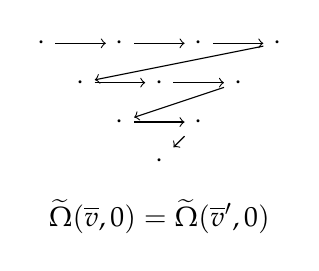
\begin{tikzpicture}
\node (41) at (-1.5,2) {$\cdot$};
\node (42) at (-0.5,2) {$\cdot$};
\node (43) at (0.5,2) {$\cdot$};
\node (44) at (1.5,2) {$\cdot$};

\node (31) at (-1,1.5) {$\cdot$};
\node (32) at (0,1.5) {$\cdot$};
\node (33) at (1,1.5) {$\cdot$};

\node (21) at (-.5,1) {$\cdot$};
\node (22) at (.5,1) {$\cdot$};

\node (11) at (0,0.5) {$\cdot$};

\node (text) at (0,-0.2) {$\widetilde\Omega(\vv, 0) = \widetilde\Omega(\vv',0)$};

\draw [->] (41) edge (42) (42) edge (43) (43) edge (44) (44) edge (31) 
	(31) edge (32) (32) edge (33) (33) edge (21) (21) edge (22) (22) edge 
	(11); 
\end{tikzpicture}
&\begin{tikzpicture}
\node (41) at (-1.5,2) {$\cdot$};
\node (42) at (-0.5,2) {$\cdot$};
\node (43) at (0.5,2) {$\cdot$};
\node (44) at (1.5,2) {$\cdot$};

\node (31) at (-1,1.5) {$\cdot$};
\node (32) at (0,1.5) {$\cdot$};
\node (33) at (1,1.5) {$\cdot$};

\node (21) at (-.5,1) {$\cdot$};
\node (22) at (.5,1) {$\cdot$};

\node (11) at (0,0.5) {$\cdot$};

\node (text) at (0,-0.2) {More examples};

\end{tikzpicture}
\end{tabular}

\end{Example}

% Recall that $z\in \DD(\vv)$ is called non-critical if $z_{k,i} \neq z_{k,j}$
% whenever $[k,i] - [k,j]$ and $k<n$.
% \begin{Lemma}
% \label{L:canonical-element}
% Every Gelfand-Tsetlin chamber contains a non-critical element.
% \end{Lemma}
% \begin{proof}
% We put a weight on each edge of $\Omega$: edges $[k,i] \rightarrow [k-1,j]$ 
% and $[n,i] \rightarrow [n,j]$ are assigned weight zero, while edges 
% $[k-1,i] \rightarrow [k,j]$ and $[k,i] \rightarrow [k,j]$ with $k<n$ are 
% assigned weight $1$. The weight of a path in $\Omega$ is the sum of the 
% weights of the edges that form the path. The \emph{depth} of a vertex $[k,i]$, 
% denoted $d([k,i])$, is the maximum of the weights of all paths from $[k,i]$ to 
% a sink of $\Omega$. Notice that if there is a path from $[n,i]$ to $[n,j]$ 
% then it must consist of arrows of weight $0$, and hence both vertices have the 
% same depth. 

% Set
% \begin{align*}
% y_{k,i}
% 	&= 
% 	\begin{cases}
% 	d([k,i]) - d([n,j]) 
% 		&\mbox{if $[k,i]$ and $[n,j]$ are connected;} \\
% 	d([k,i])
% 		&\mbox{otherwise.}
% 	\end{cases}
% \end{align*}
% By definition $y_{n,i} = 0$ for all $i \in \interval n$. Let $1 \leq i < j 
% \leq k < n$ be such that $[k,i] \rightarrow [k,j]$ in $\Omega$. By definition 
% this implies $d([k,i]) > d([k,j])$, which in turn implies $y_{k,i} > y_{k,j}$, 
% so $y \in \DD(\vv)$ and it is clearly non-critical. A similar argument shows 
% that if $[k,i] \rightarrow [k-1,j]$ in $\Omega$ then $y_{k,i} \geq y_{k-1,j}$, 
% while if $[k-1,j] \rightarrow [k,i]$ then $y_{k,i} < y_{k-1,j}$. Thus $y$ lies 
% in the same GT-chamber as $z$.
% \end{proof}
% We refer to the non-critical element found in the proof of the lemma as the
% \emph{canonical element} of the GT-chamber.
% Notice that if $[k,i] \to [l,j]$ in $\Omega(\vv,z)$ is superfluous then there 
% is a path connecting the same vertices which is formed by essential arrows, 
% and that the weigth of that path is larger than or equal to that of the edge.
% Thus the canonical element of the chamber can be found by repeating the 
% procedure of the proof with the reduced graph of $z$.

\paragraph
\about{The internal structure of the big module}
We now begin with our study of the internal structure of $V(T(\vv))$.
% \begin{Lemma}
% \label{L:same-chamber}
% Suppose $y,z \in \DD(\vv)$ lie in the same Gelfand-Tsetlin chamber. Then the
% following hold.
% \begin{enumerate}[(a)]
% \item
% \label{i:same-chamber-e}
% $U D_{e}(\vv + z) = U D_{e}(\vv+y)$

% \item
% \label{i:same-chamber-omega}
% $U D_{\omega_0^z}(\vv + z) = U D_{\omega_0^y}(\vv+y)$
% \end{enumerate}
% \end{Lemma}
% \begin{proof}
% We will prove the result taking $y$ to be the canonical element in the GT 
% chamber. Since $z$ is arbitrary, the result follows from this particular case.

% Set $\Omega = \Omega(\vv,z)$. We proceed by induction on $|y-z| = \sum_{(k,i) 
% \in \Sigma} |y_{k,i} - z_{k,i}|$. The base case is $y = z$ which is trivial. 
% If $y \neq z$ then there exists $(l,j) \in \Sigma$ such that $y_{l,j} \neq 
% z_{l,j}$. We will show that there is an element $u = z\pm \delta^{k,i} \in 
% \DD(\vv)$, in the same chamber as $y$ and $z$, such that $|y-u| = |y-z| -1$
% and such that the statement holds with $u$ instead of $y$. 

% Suppose first that $z_{l,j} < y_{l,j}$. We divide the proof in four steps. \\

% \emph{Step 1: Choosing $(k,i)$.}
% Denote by $\Omega_<$ the digraph obtained by removing from $\Omega$ those 
% vertices $[m,r]$ such that $z_{l,j} \geq y_{l,j}$. 
% Let $(k,i)$ be a source of $\Omega_<$, let $I \in \II(\vv,z)$ be such that 
% $(k,i) \in I$, and set $u = z = \delta^{k,i}$. Suppose $[k,i-1] - [k,i]$ in 
% $\Omega(\vv)$. Since the edge $[k,i-1] \rightarrow [k,i]$ is not present in 
% $\Omega_>$, it follows that $y_{k,i-1} \leq z_{k,i-1}$, and since $y$ is 
% non-critical we obtain
% \begin{align*}
% z_{k,i} < y_{k,i} < y_{k,i-1} \leq z_{k,i-1},
% \end{align*}
% which implies that $u \in \DD(\vv)$ and that $\{(k,i)\} \in \II(\vv, u)$. On 
% the other hand, if $[k,i-1]$ and $[k,i]$ are not connected by an edge in 
% $\Omega(\vv)$ the same statement holds trivially. Thus item \ref{i:omega-delta}
% of Lemma \ref{L:omega-delta} implies that $\omega_0^u = \omega_0^z 
% \alpha(I)$.\\

% \emph{Step 2: $u$ lies in the same chamber as $y$ and $z$.}
% Since we have only increased the $(k,i)$ entry of $z$ by one, it is enough to 
% check that if $[k \pm 1,j] \rightarrow [k,i]$ in $\Omega(\vv,y)$, then the 
% same edge appears in $\Omega(\vv,u)$. Since $[k,i]$ is a source in $\Omega_<$, 
% in either case we have $z_{k\pm1,j} \geq y_{k \pm 1, j}$, so
% \begin{align*}
% u_{k+1,j} 
% 	&= z_{k+1,j} \geq y_{k+1,j} \geq y_{k,i} \geq z_{k,i} + 1 = u_{k,i}, \\ 
% u_{k-1,j} &= z_{k-1,j} \geq y_{k-1,j} > y_{k,i} \geq z_{k,i} + 1 = u_{k,i},
% \end{align*}
% and hence $u$ lies in the same GT chamber as $y$ and $z$. \\

% \emph{Step 3: From $\vv+z$ to $\vv + u$.}
% Notice that the first inequality in the previous display implies that if 
% $[k,i] - [k+1,j]$ in $\Omega(\vv)$ then $z_{k,i} \neq z_{k,+1,j}$, and hence 
% $e_I(\vv+z) \neq 0$. Thus if we take the components of $E_{k,k+1} 
% D_{e}(\vv + z)$ and $E_{k,k+1} D_{\omega_0^z}(\vv + z)$ of Gelfand-Tsetlin 
% weight $\chi_{v+u}$ we obtain
% \begin{align*}
% p_{\vv+u}(E_{k,k+1} D_{e}(\vv + z))
% 	& = e_I(\vv+z) D_{\alpha(I)}(\vv + u) + D_{<\alpha(I)}(\vv + u),\\
% p_{\vv+u}(E_{k,k+1} D_{\omega_0^z}(\vv + z))
% 	& = e_{I}(\vv + z) D_{\omega_0^z \alpha(I)}(\vv + u) 
% 	+ D_{<\omega_0^z \alpha(I)}(\vv + u)
% \end{align*}
% The first equation implies that $U D_e(\vv + z) [\vv + u] \neq 0$, so by
% item \ref{i:eigenvalue} of Proposition \ref{P:gt-weight-spaces} $D_e(\vv + u)
% \in D_e(\vv + z)$. As observed above $\omega_0^z \alpha(I) = \omega_0^u$, so 
% by item \ref{i:generator} of the same proposition $D_{\omega_0^u}(\vv + u) \in 
% D_{\omega_0^z}(\vv + z)$. \\

% \emph{Step 4: From $\vv + u$ to $\vv + z$.}
% Let $J \in \II(\vv, u)$. Then either $J \in \II(\vv, z)$, or $J = 
% \interval{i+1,b(I)}_k$, or $J = \{(k,i)\}$. In each case it is easy to see 
% that $\omega_0^z$ is increasing over $J$, and so it is a $u$-shuffle. In 
% particular $D_{\omega_0^z}(\vv + u)$ is a nonzero element of $V(T(\vv))[\vv + 
% u]$. As before, we have
% \begin{align*}
% p_{\vv+z}(E_{k+1,k} D_{e}(\vv + u))
% 	&= f_{\{(k,i)\}}(\vv + u) D_e(\vv + u) \\
% p_{\vv+z}(E_{k+1,k} D_{\omega_0^z}(\vv + u))
% 	&=f_{\{(k,i)\}}(\vv + u) D_{\omega_0^z}(\vv + u) + D_{<\omega_0^z}(\vv + u)
% \end{align*}
% Now if $[k,i] \rightarrow [k-1,j]$ in $\Omega(\vv,u) = 
% \Omega(\vv,z)$, then $u_{k,i} - 1 = z_{k,i} \geq z_{k-1,j} = u_{k-1,j}$ and 
% the coefficient $f_{\{(k,i)\}}(\vv + u)$ is not zero. It follows immediately 
% that $D_e(\vv + u) \in U D_e(\vv + z)$. Again by item \ref{i:generator} of 
% Proposition \ref{P:gt-weight-spaces} we see $D_{\omega_0^z}(\vv + z) \in 
% U D_{\omega_0^u}(\vv + u)$. \\

% The case where $z_{l,j} > y_{l,j}$ can be dealt with following a similar 
% reasoning. In the first step we introduce the digraph $\Omega_>$ as that 
% obtained by deleting from $\Omega(\vv,z)$ the vertices $[m,r]$ such that 
% $z_{m,r} \leq y_{m,r}$. Then $(k,i)$ is chosen as a sink in $\Omega_>$ and $u 
% = z - \delta^{k,i}$. Steps two to four are similar to those above, mutatis 
% mutandis.
% \end{proof}
\begin{Lemma}
\label{L:omega-contained}
Let $y,z \in \DD(\vv)$. If $\Omega^+(\vv,z) \subset \Omega^+(\vv,y)$ then the
following hold.
\begin{enumerate}[(a)]
\item 
\label{i:e}
$D_{e}(\vv + y) \in U D_{e}(\vv + z)$.

\item 
\label{i:omega}
$D_{\omega_0^y}(\vv + y) \in U D_{\omega_0^z}(\vv + z)$.
\end{enumerate}
\end{Lemma}
\begin{proof}
We will proceed by induction on $|y-z| = \sum_{(k,i) \in \Sigma} |y_{k,i} - 
z_{k,i}|$, that is, we will show that it is possible to choose $(k,i) \in 
\Sigma$ and $u = z \pm \delta^{k,i}$ with the sign chosen so $|y-u|<|y-z|$, 
such that the following hold:
\begin{enumerate}
\item $u \in \DD(\vv)$.

\item $\Omega^+(\vv,z) \subset \Omega^+(\vv,u) \subset \Omega^+(\vv,y)$,

\item $D_{e}(\vv + u) \in U D_{e}(\vv + z)$, and

\item $D_{\omega_0^u}(\vv + u) \in U D_{\omega_0^z}(\vv + z)$.
\end{enumerate}
The inductive hypohtesis tells us that the statement holds with $u$ instead
of $z$, which combined with the four statements above allows us to prove
the inductive step.

Denote by $\Omega_<$, resp. $\Omega_>$, the induced subdigraph of 
$\Omega(\vv,y)$ with vertex set those $[k,i]$ such that $z_{k,i} < y_{k,i}$, 
resp. $z_{k,i} > y_{k,i}$. Notice that no vertex of the form $[n,i]$ is in 
either graph. If both $\Omega_<$ and $\Omega_>$ are empty then 
$y = z$ and there is nothing to prove. Suppose $\Omega_<$ is not empty. Then, 
since it is a subdigraph of $\Omega(\vv,y)$, it has no loops and hence has at 
least one source, say $[k,i]$. We claim that (1), (2), (3) and (4) hold with 
$u = y + \delta^{k,i}$. If $\Omega_<$ is empty then we take $[k,i]$ to be
a sink in $\Omega_>$ and set $u = y - \delta^{k,i}$. We now proceed with the 
proof of the first case, indicating how to adapt the proof for the second.

\emph{Proof of (1)}. By item \ref{i:D-delta} of Lemma \ref{L:omega-delta}
it is enough to show that if $[k,i-1] - [k,i]$ is an edge of $\Omega(\vv)$ 
then $z_{k,i-1} > z_{k,i}$. If this edge is indeed present then $[k,i-1] \to 
[k,i]$ is an edge of $\Omega^+(\vv,y)$, and since $[k,i]$ is a source of 
$\Omega_<$ it follows that $z_{k,i-1} \geq y_{k-1,i}$. On the other hand
$y_{k,i-1} \geq y_{k,i} > z_{k,i}$, so $z_{k,i-1} > z_{k,i}$. The proof in
the other case is analogous.

\emph{Proof of (2).} To show that $\Omega^+(\vv,z) \subset \Omega^+(\vv,u)$ 
it is enough to prove that if $[k,i] \to [k-1,j]$ or $[k+1,j] \to [k,i]$ are 
edges of $\Omega(\vv,z)$ then they are also edges of $\Omega^+(\vv,u)$. The 
first case is obvious. For the second, the choice of $(k,i)$ as a source of 
$\Omega_<$ implies that $z_{k+1,j} = u_{k+1,j} \geq y_{k+1,j}$ while $u_{k,i}
= z_{k,i} + 1 \leq y_{k,i}$. Since $\Omega^+(\vv,z) \subset \Omega^+(\vv,y)$
we see that $u_{k+1,j} \geq y_{k+1,j} \geq y_{k,i} \geq u_{k,i}$, so the edge
$[k+1,j] \to [k,i]$ is in $\Omega^+(\vv,u)$.

To show that $\Omega^+(\vv, u) \subset \Omega^+(\vv, y)$ we again need to 
consider only edges of the form $[k+1,j] \to [k,i]$ and $[k,i] \to [k-1,j]$ 
of the first graph. In the first case we have $z_{k+1,j} = u_{k+1,j} \geq
u_{k,i} = z_{k,i} + 1$, so $[k+1,j] \to [k,i]$ is an edge of $\Omega^+(\vv,z)$,
and hence in $\Omega^+(\vv,y)$. In the second case we have that $z_{k,i} +1 =
u_{k,i} \geq u_{k-1,j} = z_{k-1,j}$. If the inequality is strict then $[k,i]
\to [k-1,j]$ is an edge of $\Omega^+(\vv,z)$, and hence in $\Omega^+(\vv,y)$.
The alternative is that $z_{k,i} + 1 = z_{k-1,j}$, in which case $[k-1,j]
\to [k,i]$ is an edge of $\Omega^+(\vv,z)$ and hence of $\Omega^+(\vv,y)$. 
Since $(k,i)$ is a soure of $\Omega_<$ this means that $y_{k-1,j} \leq 
z_{k-1,j} = z_{k,i} + 1 \leq y_{k,i}$, so $[k,i] \to [k-1,j]$ is an edge of 
$\Omega^+(\vv,y)$. The proof in the second case is analogous.

\emph{Proof of (3).} Let $I \in \II(\vv,z)$ be the interval containing 
$(k,i)$. It follows from the definitions that $\alpha(I)$ is a $u$-shuffle.
Using the formulas in Theorem \ref{T:gt-big-module} we see that
\begin{align*}
p_{\vv+u}&(E_{k,k+1} D_e(\vv + z)) =\\
	&e_I(\vv + z) D_{\alpha(I)}(\vv + u) + D_{<\alpha(I)}(\vv + u),
\end{align*}
and by Lemma \ref{L:sub-gt} this element lies in $U D_e(\vv + z)$. 

We now prove, by contradiction, that $e_I(\vv + z) \neq 0$. If it were $0$
then there would exist some $(k+1,j) \in \Sigma$ such that $z_{k+1,j} = 
z_{k,i}$, which would imply that $[k+1,j] \to [k,i]$ is an edge of 
$\Omega^+(\vv, z)$ and hence that $y_{k+1,j} \geq y_{k,i}$. On the other hand
since $(k,i)$ is a source of $\Omega_<$ we have $z_{k+1,j} \geq y_{k+1,j} \geq 
y_{k,i} > z_{k,i}$, a contradiction. 
Thus we see that $p_{\vv+u}(E_{k,k+1} D_e(\vv + z)) \neq 0$. By item 
\ref{i:eigenvalue} of Proposition \ref{P:gt-weight-spaces} this implies that
$D_e(\vv + u) \in U D_e(\vv + z)$. The proof in the second case is analogous,
except that we must look at $p_u(E_{k+1,k} D_e(\vv + z))$, and instead of 
$e_I(\vv+z)$ one must show that $f_I(\vv + z)$ is nonzero.

\emph{Proof of (4).} Recall from item \ref{i:omega-delta} of Lemma
\ref{L:omega-delta} that there exists $\sigma \in S_\pi^z$ such that 
$\omega_0^u = \sigma\alpha(I)$. By item \ref{i:generator} of Proposition 
\ref{P:gt-weight-spaces} $D_\sigma(\vv + z) \in U D_{\omega_0^z}(\vv + z)$.
Again by the formulas in \ref{T:gt-big-module} and by Lemma \ref{L:sub-gt} 
\begin{align*}
p_{\vv+u}&(E_{k,k+1} D_\sigma(\vv + z)) =\\
	&e_I(\vv + z) D_{\sigma\alpha(I)}(\vv + u) + D_{<\alpha(I)}(\vv + u)
	\in U D_{\omega_0^z},
\end{align*}
and item \ref{i:generator} of Proposition \ref{P:gt-weight-spaces} implies
that this element generates the GT weight component $V(T(\vv))[\vv + u]$, so 
in particular $D_{\omega_0^u}(\vv + u) \in U D_{\omega_0^z}(\vv + z)$. For the 
second case we must take $p_{\vv+u}(E_{k,k+1} D_\tau(\vv + z))$, with 
$\tau$ as in item \ref{i:omega-delta} of Lemma \ref{L:omega-delta}, and the 
rest of the proof is similar.
\end{proof}

\paragraph
\about{Cyclic submodules}
Recall that $z \in \DD(\vv)$ is said to be \emph{fully critical} if $[k,i] - 
[k,j]$ implies $z_{k,i} = z_{k,j}$. The following proposition shows that 
$V(T(\vv))$ is a cyclic module, and that it has a unique minimal module. For 
this we point out that there always exist fully critical $z \in \DD(\vv)$ 
such that $\Omega^-(\vv,z) = \emptyset$ or $\Omega^+(\vv,z) = \emptyset$.
\begin{Proposition}
\label{P:cyclic}
Let $z \in \DD(\vv)$ fully critical.
\begin{enumerate}[(a)]
\item 
\label{i:cyclic}
If $\Omega^+(\vv, z)$ is empty then $U D_e(\vv + z) = V(T(\vv))$.

\item
\label{i:minimal-module}
If $\Omega^-(\vv,z)$ is empty then $U D_e(\vv + z)$ is simple, and coincides 
with the socle of $V(T(\vv))$.

\item
\label{i:simple}
If there are no edges of the form $[k,i] - [k-1,j]$ in $\Omega(\vv)$ then
$V(T(\vv))$ is simple.
\end{enumerate}
\end{Proposition}
\begin{proof}
Since $z$ is fully critical $\omega_0^z = e$. If $\Omega^+(\vv + z) = 
\emptyset$ then by item \ref{i:omega} of Lemma \ref{L:omega-contained} every
tableaux $D_{\omega_0^y}(\vv + y)$ with $y \in \DD(\vv)$ is in $U D_e(\vv+z)$.
Thus 
\[
U D_e(\vv+z)[\vv + y] 
	\supset \Gamma D_{\omega_0^y}(\vv+y) 
	= V(T(\vv))[\vv+y]
\]
and this proves item \ref{i:cyclic}.

Assume $\Omega^-(\vv,z) = \emptyset$ and set $N = U D_e(\vv + z)$. Then 
for any $y \in \DD(\vv)$ we have $\Omega^+(\vv,y) \subset \Omega^+(\vv,z)$ so
by item \ref{i:e} of Lemma \ref{L:omega-contained} $N \subset U D_e(\vv + y)$.
Since every submodule of $V(T(\vv))$ contains some tableaux of this form, it
follows that $N$ is contained inside every submodule of $V(T(\vv))$ which 
proves item \ref{i:minimal-module}. Item \ref{i:simple} follows from the 
previous two.
\end{proof}

\textcolor{red}{This proposition suggests that we should study submodules of 
the form $U D_e(\vv+z)$ with $z$ fully critical such that neither 
$\Omega^+(\vv,z)$ nor $\Omega^-(\vv,z)$ is empty. \textbf{Conjecture:} If $z,y$
are fully critical and $\Omega^+(\vv,z) \subsetneq \Omega^+(\vv,y)$ then 
$UD_e(\vv + y) \subsetneq UD_e(\vv + z)$.}

\paragraph
\about{The socle of $V(T(\vv))$}
For the rest of this section we denote by $N = N(\vv)$ the socle of $V$. As 
mentioned above $N$ is simple. Recall also that the dimension of the GT 
component $N[\vv+z] \subset V[\vv+z]$ is bounded by $|S_\pi^z|$.
\begin{Definition}
Let $z \in \DD$. We say that $\vv + z$ is in the \emph{essential support} of 
$N$ if $\dim N[\vv+z] = |S_\pi|$. We denote by $\essupp(\vv)$ the set of all
$z \in \DD(\vv)$ such that $\vv + z$ lies in the essential support of $N$.
\end{Definition}

If $\vv + z$ is in the essential support of $N$ then necessarily $z$ is 
non-critial. Also, if $y \in \DD$ and $\Omega^+(\vv,z) \subset \Omega^+(\vv,y)$
then Lemma \ref{L:omega-contained} implies that $\vv + y$ is also in the
essential support of $N$. Set 
\begin{align*}
	\mathcal P = \{\Omega^+(\vv,z) \mid z \in \essupp(\vv)\}. 
\end{align*} 
Then $\mathcal P$ is a finite poset with respect to the property of being a
subgraph, and hence has a set of maximal elements which we denote by 
$\mathcal P_0$. We thus have
\begin{align*}
\essupp(\vv)
	&= \bigcup_{\Omega \in \mathcal P} \{z \in \essupp(\vv) \mid \Omega = 
		\Omega^+(\vv,z)\} \\
	&= \bigcup_{\Omega \in \mathcal P_0} \{z \in \essupp(\vv) \mid \Omega 
		\subset \Omega^+(\vv,z)\}
\end{align*}

Denote by $\RR^\mu$ the set of points in $\CC^\mu$ with real coordinates. 
Recall that a rational polyhedral cone is the intersection of finitely many
half-spaces $\{x \in \RR^\mu \mid \phi(x) \geq q\}$ where $\phi$ is a 
functional with rational coefficients in the canonical basis and $q \in \QQ$. 
Also recall that a point in a rational polyhedral cone is called integral if 
all its coordinates are integral.
\begin{Lemma}
\label{L:essupp-polyhedra}
Let $\Omega \in \mathcal P$. Then the sets $\{z \in \essupp(\vv) \mid \Omega = 
\Omega^+(\vv,z)\}$ and $\{z \in \essupp(\vv) \mid \Omega \subset 
\Omega^+(\vv,z)\}$ are nonempty sets consisting of the integral points of 
rational polyhedral cones in $\RR^\mu$.
\end{Lemma}
\begin{proof}
Consider the following set of inequalities:
\begin{enumerate}[$(a)$]
\item $z_{n-1,j} \leq \vv_{n,i} - \vv_{n-i,j}$ whenever $[n,i] \to [n-1,j]$ is
a vertex of $\Omega$;

\item $z_{n-1,j} > \vv_{n,i} - \vv_{n-i,j}$ whenever $[n-1,j] \to [n,i]$ is
a vertex of $\Omega$;

\item $z_{k-1,j} \leq z_{k,j}$ whenever $k < n$ and $[k,i] \to [k-1,j]$ is
a vertex of $\Omega$;

\item $z_{k-1,j} > z_{k,j}$ whenever $k < n$ and $[k-1,i] \to [k,j]$ is
a vertex of $\Omega$;

\item $z_{k,i} > z_{k,i+1}$ whenever $k<n$ and $[k,i] \to [k,i+1]$ is a vertex
of $\Omega$.
\end{enumerate}
An element $z \in \ZZ^\mu$ satisfies these five inequalities if and only if it 
is a noncritical element of $\DD$ such that $\Omega(\vv,z) = \Omega$, or 
equivalently if it belongs to $\{z \in \essupp(\vv) \mid \Omega = 
\Omega^+(\vv,z)\}$, so by definition this set is the set of integral points of 
a rational polyhedral cone, which is nonempty by definition of $\mathcal P$. A 
similar reasoning works for the set $\{z \in \essupp(\vv) \mid \Omega \subset 
\Omega^+(\vv,z)\}$, but in that case we need only consider points satisfying 
inequalities $(a), (c), (e)$.
\end{proof}

As seen in Proposition \ref{P:cyclic}, $N$ is generated by $D_e(\vv)$ and 
by Lemma \ref{L:omega-contained} it contains any element of the form 
$D_{\omega_0^z}(\vv + z)$ such that $\Omega(\vv,z) = \Omega(\vv,0)$. Now if we
put $\Omega = \Omega(\vv,0)$ in the list of inequalities $(a), (b), (c), (d), 
(e)$ from the previous proof, the solutions form a rational cone of dimension
$\dim \RR^\mu = \frac{n(n-1)}{2}$. We thus have the following result.

\begin{Proposition}
\label{P:essupp}
The essential support of $N$ is a union of sets of integral points of rational 
polyhedral cones. Furthermore, at least one of these polyhedral cones has 
dimension $\frac{n(n-1)}{2}$.
\end{Proposition}

\paragraph
\about{Verma modules and their tableaux realizations}

Let $\lambda = (\lambda_1, \ldots, \lambda_n) \in \CC^n$. We define 
$\widetilde HW(\lambda) \in \CC^\mu$ to be the point with coordinates 
$\widetilde HW(\lambda)_{k,i} = \lambda_{n-k+i} + i - k$. Set $HW(\lambda)$
to be an element in normal form in the $S_\mu$-orbit of $\widetilde 
HW(\lambda)$ and fix $\vv$ a seed in the class of $HW(\lambda)$. 

The derived talbeau $D_e(HW(\lambda))$ is a highest weight vector in 
$V(T(\vv))$, of weight $\lambda$. Thus if we take the corresponding Verma 
module $M(\lambda)$, we obtain a natural map $M(\lambda) \to V(T(\vv))$ 
sending a highest weight vector $v_\lambda$ to $D_e(HW(\lambda))$. 

\textcolor{red}{
\begin{Lemma}
Let $\lambda \in \CC^n$ and let $\vv$ be a seed in the class of $HW(\lambda)$.
Then the map $j_\lambda: L(\lambda) \to V(T(\vv))$ is injective.
\end{Lemma}
\begin{proof}
SKETCH: $L(\lambda)$ has a unique minimal submodule $L(\mu)$, so if $j_\lambda$
is not injective we have $L(\mu) \subset \ker j_\lambda$, and the image of
$j_\lambda$ can not contain a highest weight vector of weight $\mu$. 
But the image of $j_\lambda$ is $U D_e(HW(\lambda))$ and so if we can show 
that $\Omega^+(HW(\lambda)) \subset \Omega^+(HW(\mu))$ then $D_e(HW(\mu))$ 
lies in the image of $j_\lambda$, a contradiction. 
\end{proof}
}

\textcolor{red}{
Consequence: Every Verma is a submodule of $V(T(\vv))$ for the right $\vv$, and
hence every minimal Verma is the socle of that big module, so we can apply
Proposition \ref{P:essupp} 
}
\begin{bibdiv}
\begin{biblist}
\bibselect{references}
\end{biblist}
\end{bibdiv}

\newpage
\section*{Summary of results}

We fix a seed $\vv \in \CC^\mu$. We denote by $\Omega^+(\vv + z)$ the digraph 
with vertex set $\{[k,i] \mid 1 \leq i \leq k \leq n\}$, with an edge of 
the form $[k,i] \to [k-1,j]$ if and only if $\vv_{k,i} + z_{k,i} - \vv_{k-1,j} 
- z_{k-1,j} \in \ZZ_{\geq 0}$. Analogously $\Omega^-(\vv + z)$ is the digraph 
with the same vertex set and edges of the form $[k,i] \to [k-1,j]$ if and only 
if $\vv_{k,i} + z_{k,i} - \vv_{k-1,j} - z_{k-1,j} \in \ZZ_{< 0}$.

\begin{Proposition*}
Let $\vv + z$ be fully critical.
If $\Omega^+(\vv, z) = \emptyset$ then $V(T(\vv)) = U D_e(\vv + z)$. On the 
other hand, if  $\Omega^-(\vv, z) = \emptyset$ then $U D_e(\vv + z)$ is the 
socle of $V(T(\vv))$, which is simple. Furthermore, if $\Omega^-(\vv, y) = 
\emptyset$ then $\operatorname{soc} (V(T(\vv))) [\vv + y]= V(T(\vv))[\vv + y]$.
\end{Proposition*}

\begin{Example*}
\textbf{The Verma module $V(-\rho)$.} Set $n = 4$, let $\vv = \mathbf{0} 
\in \CC^\mu$, and let $V = V(T(\vv))$. Then 

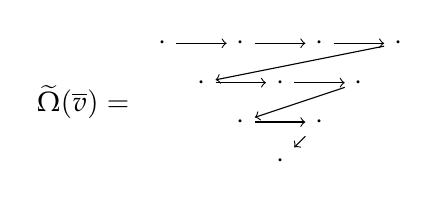
\begin{tikzpicture}
\node (v) at (-2.5,1.25) {$\widetilde\Omega(\vv) = $};

\node (41) at (-1.5,2) {$\cdot$};
\node (42) at (-0.5,2) {$\cdot$};
\node (43) at (0.5,2) {$\cdot$};
\node (44) at (1.5,2) {$\cdot$};

\node (31) at (-1,1.5) {$\cdot$};
\node (32) at (0,1.5) {$\cdot$};
\node (33) at (1,1.5) {$\cdot$};

\node (21) at (-.5,1) {$\cdot$};
\node (22) at (.5,1) {$\cdot$};

\node (11) at (0,0.5) {$\cdot$};

\draw [->] (41) edge (42) (42) edge (43) (43) edge (44) (44) edge (31) 
	(31) edge (32) (32) edge (33) (33) edge (21) (21) edge (22) (22) edge (11);
\end{tikzpicture}

\noindent so $\Omega^-(\vv) = \emptyset$. 

By the Gelfand-Tsetlin formulas $D_e(\vv)$ is a highest weight vector of 
weight $(0,1,2,3)$; notice that if we restrict the action to 
$\mathfrak{sl(4,\CC)}$ this is a highest weight vector of weight $-\rho = 
(-1,-1,-1)$. The socle of $V$ is the cyclic module generated by $D_e(\vv)$, 
which is a quotient of the Verma module $V(-\rho)$; since this is a simple 
Verma module it follows that $\operatorname{soc}(V(T(\vv))) = U D_e(\vv) \cong 
V(-\rho)$. Now let

\begin{tikzpicture}
\node (v) at (-2.5,1.25) {$y = $};

\node (41) at (-1.5,2) {$0$};
\node (42) at (-0.5,2) {$0$};
\node (43) at (0.5,2) {$0$};
\node (44) at (1.5,2) {$0$};

\node (31) at (-1,1.5) {$0$};
\node (32) at (0,1.5) {$-1$};
\node (33) at (1,1.5) {$-2$};

\node (21) at (-.5,1) {$-2$};
\node (22) at (.5,1) {$-3$};

\node (11) at (0,0.5) {$-3$};
\end{tikzpicture}

This is the canonical element in the Gelfand-Tsetlin chamber of $\vv$, and 
hence $\dim V(-\rho)[y] = \dim V(T(\vv))[y] = 3!2!$. Thus there exists a simple
GT module with the maximal GT multiplicity possible for the character $\chi_y$.
Similar considerations apply for $n$ arbitrary.
\end{Example*}

\begin{Example*}
\textbf{The Verma module $V(-2\rho)$.} Take as seed

\begin{tikzpicture}
\node (v) at (-2.5,1.25) {$\vv = $};

\node (41) at (-1.5,2) {$3$};
\node (42) at (-0.5,2) {$2$};
\node (43) at (0.5,2) {$1$};
\node (44) at (1.5,2) {$0$};

\node (31) at (-1,1.5) {$0$};
\node (32) at (0,1.5) {$0$};
\node (33) at (1,1.5) {$0$};

\node (21) at (-.5,1) {$0$};
\node (22) at (.5,1) {$0$};

\node (11) at (0,0.5) {$0$};
\end{tikzpicture}

Inside $V = V(T(\vv))$ we find a copy of the Verma module $V(-2\rho)$ by taking
$z$ as below (we have also drawn the corresponding reduced graph).

\begin{tikzpicture}
\node (v) at (-2.5,1.25) {$z = $};

\node (41) at (-1.5,2) {$0$};
\node (42) at (-0.5,2) {$0$};
\node (43) at (0.5,2) {$0$};
\node (44) at (1.5,2) {$0$};

\node (31) at (-1,1.5) {$2$};
\node (32) at (0,1.5) {$1$};
\node (33) at (1,1.5) {$0$};

\node (21) at (-.5,1) {$1$};
\node (22) at (.5,1) {$0$};

\node (11) at (0,0.5) {$0$};
\end{tikzpicture}
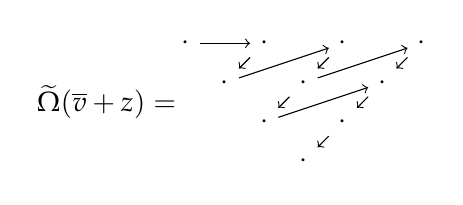
\begin{tikzpicture}
\node (v) at (-2.5,1.25) {$\widetilde\Omega(\vv+z) = $};

\node (41) at (-1.5,2) {$\cdot$};
\node (42) at (-0.5,2) {$\cdot$};
\node (43) at (0.5,2) {$\cdot$};
\node (44) at (1.5,2) {$\cdot$};

\node (31) at (-1,1.5) {$\cdot$};
\node (32) at (0,1.5) {$\cdot$};
\node (33) at (1,1.5) {$\cdot$};

\node (21) at (-.5,1) {$\cdot$};
\node (22) at (.5,1) {$\cdot$};

\node (11) at (0,0.5) {$\cdot$};

\draw [->] (41) edge (42) (42) edge (31) (31) edge (43) (43) edge (32) 
	(32) edge (44) (44) edge (33) (32) edge (21) (21) edge (33) (33) edge (22)
	(22) edge (11);
\end{tikzpicture}

In this case $\vv+z$ is the canonical element in its own GT chamber and 
$D_e(\vv+z)$ is a highest weight vector with $\mathfrak{sl}(4,\CC)$-weight 
$-2\rho = (-2,-2,-2)$, so $V(-2\rho) \cong U D_e(\vv+z)$. This is again a 
simple module so $\operatorname{soc}(V) = V(-2\rho)$. Since $\vv$ is a seed we 
have $\operatorname{soc}(V) = U D_e(\vv)$. Thus $\Omega^+(\vv + z) \subsetneq 
\Omega^+(\vv)$ but $U D_e(\vv) = U D_e(\vv + z)$. Now the canonical element 
inside the GT chamber of $\vv$ is
\end{Example*}
\end{document}

